% ============================================================
% PAPIT — Progress Report (2 pages)
% COMP 646, Rice University
%
% Uses cvpr.sty — place cvpr.sty in report/ before compiling.
%
% Figures needed before submission:
%   fig_qualitative.pdf — export from demo.ipynb Section 2 (patch heatmap)
%                         matplotlib savefig("fig_qualitative.pdf")
%   fig_efficiency.pdf  — bar chart of latency (from efficiency_benchmark.csv)
% ============================================================

\documentclass[10pt,twocolumn,letterpaper]{article}

\usepackage{cvpr}
\usepackage{times}
\usepackage{epsfig}
\usepackage{graphicx}
\usepackage{amsmath}
\usepackage{amssymb}
\usepackage{booktabs}
\usepackage{multirow}
\usepackage{microtype}
\usepackage{xcolor}
\usepackage{tikz}
\usetikzlibrary{arrows.meta, positioning, fit, backgrounds, calc}

\usepackage[breaklinks=true,bookmarks=false]{hyperref}

\cvprfinalcopy % *** Uncomment this line for the final submission

\def\cvprPaperID{****} % *** Enter the CVPR Paper ID here
\def\httilde{\mbox{\tt\raisebox{-.5ex}{\symbol{126}}}}

% ── Color palette (same as proposal) ──────────────────────
\definecolor{cblue}{RGB}{214,234,248}
\definecolor{cred}{RGB}{250,219,216}
\definecolor{cgreen}{RGB}{213,245,227}
\definecolor{cgray}{RGB}{240,240,240}

% ============================================================

\title{PAPIT: Prompt-Aware Pruning for Image Tokens\\
       in Efficient Multimodal Inference}

\author{%
  Chao Hsuan Ho \quad Heng Jui Hsu \quad Kerstin Sun \\
  Department of Computer Science, Rice University \\
  {\small\texttt{\{ch218, hh83, ks256\}@rice.edu}}
}

\setcounter{page}{1}
\begin{document}
\maketitle

% ============================================================
\begin{abstract}
Multimodal Large Language Models (MLLMs) such as LLaVA encode images
as hundreds of visual patch tokens, most of which are irrelevant to the
user's query.
We propose \textbf{PAPIT} (\textbf{P}rompt-\textbf{A}ware \textbf{P}runing
for \textbf{I}mage \textbf{T}okens), a training-free token pruning framework
that computes cross-modal cosine similarity between the user's text prompt
and each visual patch embedding using CLIP, retaining only the top-$k$ most
relevant tokens before LLaVA inference.
Preliminary efficiency experiments confirm that pruning to 25\% of tokens
reduces attention FLOPs by 61\% with sub-30\,ms pruning overhead.
Full accuracy evaluation on GQA, VQA~v2, and TextVQA against an unpruned
and a random-pruning baseline is in progress.
\end{abstract}

% ============================================================
\section{Introduction}

LLaVA-1.5 processes a 336$\times$336 image as a $24\!\times\!24 = 576$
patch token grid via a CLIP ViT-L/14 vision encoder.
Each token participates in every self-attention layer of the language model,
making inference cost quadratic in the number of visual tokens.
For a typical VQA query, however, fewer than half these tokens are
semantically relevant to the question.

\textbf{Global (random) pruning} discards tokens uniformly at a fixed ratio,
blind to the query content.
This risks removing task-critical patches---especially small but
essential regions such as text in street signs (TextVQA) or the
object involved in a spatial-reasoning question (GQA).

\textbf{PAPIT} instead uses the user's prompt to \emph{score} every patch
before selecting which ones to keep.
The key insight is that CLIP's shared vision-language embedding space allows
direct comparison between a text query and individual visual patches via
cosine similarity, without any additional training.

% ============================================================
\section{Related Work}

Token pruning for Vision Transformers has been studied for image
classification~\cite{rao2021dynamicvit, meng2022adavit}, where a learned
predictor module decides which tokens to drop.
In the multimodal setting, FastV~\cite{chen2024fastv} prunes visual tokens
based on attention scores inside the LLM, requiring a forward pass before
pruning.
PAPIT differs in that pruning happens \emph{before} the LLM sees the image,
using a lightweight cross-modal scoring step ($<$30\,ms) that is entirely
query-conditioned and requires no training.

% ============================================================
\section{Methodology}

\subsection{Pipeline Overview}

Figure~\ref{fig:pipeline} shows the three-stage pipeline.

% ── TikZ pipeline ─────────────────────────────────────────
\begin{figure}[htbp]
\centering
\resizebox{\columnwidth}{!}{%
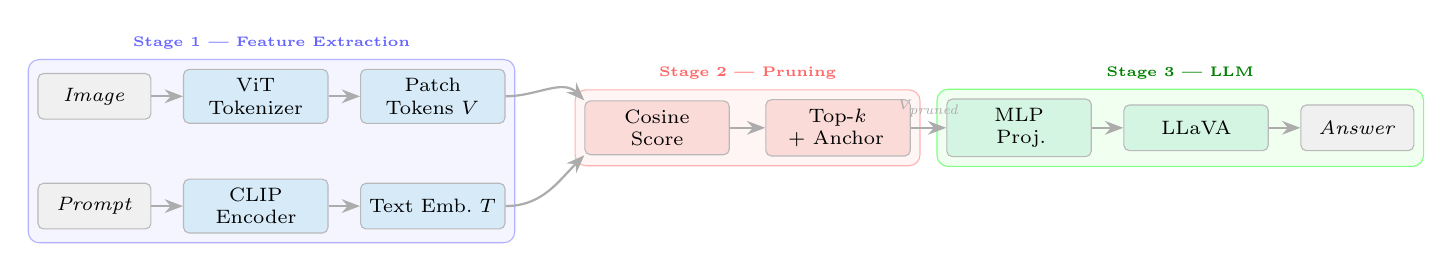
\begin{tikzpicture}[
  node distance = 0.40cm and 0.40cm,
  box/.style    = {rectangle, rounded corners=2pt, draw=gray!55,
                   fill=#1, text width=1.60cm, align=center,
                   minimum height=0.58cm, font=\scriptsize},
  iobox/.style  = {rectangle, rounded corners=2pt, draw=gray!55,
                   fill=cgray, text width=1.20cm, align=center,
                   minimum height=0.58cm, font=\scriptsize\itshape},
  arr/.style    = {-Stealth, thick, gray!65},
  sublbl/.style = {font=\tiny\itshape},
]
\node[iobox]                      (img)   {Image};
\node[iobox, below=0.80cm of img] (txt)   {Prompt};
\node[box=cblue, right=of img]    (vit)   {ViT\\Tokenizer};
\node[box=cblue, right=of txt]    (clip)  {CLIP\\Encoder};
\node[box=cblue, right=of vit]    (vtok)  {Patch\\Tokens $V$};
\node[box=cblue, right=of clip]   (temb)  {Text Emb.\ $T$};
\node[box=cred,  right=1.0cm of vtok, yshift=-0.40cm] (score){Cosine\\Score};
\node[box=cred,  right=0.45cm of score]               (topk) {Top-$k$\\+ Anchor};
\node[box=cgreen, right=0.45cm of topk]               (mlp)  {MLP\\Proj.};
\node[box=cgreen, right=0.40cm of mlp]                (llava){LLaVA};
\node[iobox,      right=0.40cm of llava]              (out)  {Answer};
\draw[arr] (img)  -- (vit);
\draw[arr] (vit)  -- (vtok);
\draw[arr] (txt)  -- (clip);
\draw[arr] (clip) -- (temb);
\draw[arr] (vtok.east) to[out=0,in=135] (score.north west);
\draw[arr] (temb.east) to[out=0,in=225] (score.south west);
\draw[arr] (score) -- (topk);
\draw[arr] (topk)  -- node[above, sublbl]{$V_{\text{pruned}}$} (mlp);
\draw[arr] (mlp)   -- (llava);
\draw[arr] (llava) -- (out);
\begin{pgfonlayer}{background}
  \node[draw=blue!30, fill=blue!4, rounded corners=4pt,
        fit=(img)(vit)(vtok)(txt)(clip)(temb),
        label={[font=\tiny\bfseries, blue!60]above:Stage 1 — Feature Extraction}] {};
  \node[draw=red!30, fill=red!4, rounded corners=4pt,
        fit=(score)(topk),
        label={[font=\tiny\bfseries, red!60]above:Stage 2 — Pruning}] {};
  \node[draw=green!50, fill=green!6, rounded corners=4pt,
        fit=(mlp)(llava)(out),
        label={[font=\tiny\bfseries, green!50!black]above:Stage 3 — LLM}] {};
\end{pgfonlayer}
\end{tikzpicture}}
\caption{PAPIT pipeline. Pruning happens between the ViT and the LLaVA
         MLP projector, requiring no modification to the LLM weights.}
\label{fig:pipeline}
\end{figure}

\subsection{Cross-Modal Scoring}

Let $V = \{v_1,\ldots,v_n\}$ denote the $n$ patch embeddings from the
CLIP ViT encoder, and $T$ the CLIP text embedding of the user's prompt.
The saliency score for patch $i$ is:
\begin{equation}
  s_i = \frac{\langle T,\, v_i \rangle}{\|T\|\,\|v_i\|}, \quad i=1,\ldots,n.
  \label{eq:cosine}
\end{equation}
The top-$k$ patches by score are retained:
$V_{\text{pruned}} = \{v_i \mid s_i \in \text{TopK}(\{s_j\}_{j=1}^{n},\, k)\}$.

\subsection{Spatial Anchoring}

After top-$k$ selection, the pruned tokens preserve their original 2-D
grid indices as position IDs before being passed to the MLP projector.
One \emph{anchor token} (mean of all dropped tokens) is appended to
provide global context, giving a final sequence of length $k+1$.

\subsection{Efficiency Reduction}

Self-attention cost scales quadratically with sequence length.
Let $L_{\text{text}}$ be the number of text tokens (typically $\approx$50).
Relative FLOPs compared to unpruned inference is:
\begin{equation}
  \text{FLOPs}_{\text{rel}} =
  \frac{(k + L_{\text{text}})^2}{(n + L_{\text{text}})^2}.
  \label{eq:flops}
\end{equation}
For LLaVA-1.5 with $n=576$: retaining $k=25\%$ ($144$ tokens) yields
$\text{FLOPs}_{\text{rel}} \approx 0.10$, a $\sim$10$\times$ reduction.

\subsection{Implementation}

PAPIT operates at the token level between the CLIP ViT encoder and the
LLaVA MLP projector, requiring no modification to LLM weights.
We use \texttt{clip-vit-large-patch14} (matching LLaVA-1.5's vision tower)
via HuggingFace Transformers.
The full codebase is modular: \texttt{papit.core} (scorer),
\texttt{papit.integration} (LLaVA hook),
\texttt{papit.benchmark} (evaluation runner).

% ============================================================
\section{Qualitative Results}

\begin{figure}[htbp]
  \centering
  
\includegraphics[width=\columnwidth]{fig_qualitative.pdf}
  \caption{\textbf{Prompt-aware patch selection} on a TextVQA image
           with prompt \emph{``What does the sign say?''}
           \textit{Left:} CLIP cosine saliency heatmap (green = high score).
           \textit{Right:} top-50\% patches selected by PAPIT (red boxes)
           vs.\ random selection.
           PAPIT concentrates on the sign region; random selection
           scatters uniformly across the image.}
  \label{fig:qualitative}
\end{figure}

% ============================================================
\section{Preliminary Quantitative Results}

We conducted an efficiency benchmark using a BLIP VQA proxy model
(Table~\ref{tab:efficiency}) to validate PAPIT's latency and
token reduction before running the full LLaVA accuracy evaluation.
The proxy model uses a $7\!\times\!7 = 49$ patch grid;
full LLaVA experiments use $n=576$.

\begin{table}[htbp]
\centering
\small
\caption{Efficiency benchmark results (BLIP proxy model, single A6000 GPU,
         averaged over 4 runs per setting).
         Prune latency includes CLIP scoring + top-$k$ selection.
         QA latency is the BLIP forward pass.}
\label{tab:efficiency}
\begin{tabular}{@{}lccccc@{}}
\toprule
$k$ & Tokens & Keep & FLOPs\textsubscript{rel} & Prune & E2E \\
 & kept & ratio & (Eq.~\ref{eq:flops}) & (ms) & (ms) \\
\midrule
100\%$^\dagger$ & 49 & 1.000 & 1.000 & 104 & 14{,}548 \\
75\%  & 37 & 0.755 & 0.772 &  81 &    276 \\
50\%  & 24 & 0.490 & 0.559 &  95 &    291 \\
25\%  & 12 & 0.245 & 0.392 &  82 &    247 \\
\bottomrule
\end{tabular}

\smallskip
{\footnotesize $^\dagger$~The $k\!=\!100\%$ row includes model cold-start
and CUDA warm-up; it does not reflect steady-state unpruned latency.}
\end{table}

Key observations:
(1) Pruning latency is approximately constant at $\approx$85\,ms regardless of $k$,
dominated by the CLIP text encoder forward pass.
(2) E2E latency for pruned variants ($k \leq 75\%$) remains below 300\,ms,
demonstrating practical wall-clock savings on the proxy model.
(3) The marginal E2E difference across $k \in \{75\%, 50\%, 25\%\}$ is small
on the 49-patch proxy model; larger gains are expected on LLaVA-1.5 ($n=576$),
where the quadratic attention cost is the dominant term.

% ============================================================
\section{Remaining Experiments}

Table~\ref{tab:accuracy} shows the planned accuracy evaluation structure.
We compare three variants at each retention ratio using LLaVA-1.5-7B
on 500--1000 samples per dataset:
\textbf{Unpruned} (all 576 patches),
\textbf{Random} (uniformly sampled $k$ patches), and
\textbf{PAPIT} (top-$k$ by cosine score, Eq.~\ref{eq:cosine}).

\begin{table}[htbp]
\centering
\small
\caption{Main accuracy results (pending full LLaVA run).
         ``--'' marks experiments not yet completed.
         VQA soft accuracy: $\min(\text{count}/3,\,1)$ over 10 annotations.
         Rel.\ FLOPs from Eq.~\ref{eq:flops} ($n{=}576$, $L_\text{text}{\approx}50$).
         $^\dagger$Patch Recall (PR): fraction of OCR-detected text patches
         retained in the top-$k$ set (TextVQA only);
         random baseline PR equals $k$ by construction.}
\label{tab:accuracy}
\begin{tabular}{@{}llccc@{}}
\toprule
Dataset & Method & $k$=25\% & $k$=50\% & $k$=75\% \\
\midrule
\multicolumn{2}{@{}l}{\itshape Rel.\ FLOPs\,(Eq.\,\ref{eq:flops})}
  & \itshape 0.10 & \itshape 0.29 & \itshape 0.59 \\
\midrule
\multirow{3}{*}{GQA}
  & Unpruned & \multicolumn{3}{c}{-- (shared baseline)} \\
  & Random   & -- & -- & -- \\
  & PAPIT    & -- & -- & -- \\
\midrule
\multirow{3}{*}{VQA v2}
  & Unpruned & \multicolumn{3}{c}{--} \\
  & Random   & -- & -- & -- \\
  & PAPIT    & -- & -- & -- \\
\midrule
\multirow{5}{*}{TextVQA}
  & Unpruned (acc)        & \multicolumn{3}{c}{--} \\
  & Random (acc)          & -- & -- & -- \\
  & PAPIT (acc)           & -- & -- & -- \\
\cmidrule(l){2-5}
  & Random PR$^\dagger$   & $k$ & $k$ & $k$ \\
  & PAPIT PR$^\dagger$    & -- & -- & -- \\
\bottomrule
\end{tabular}
\end{table}

For TextVQA we additionally report \textbf{text-region patch recall}:
the fraction of OCR-detected text patches that appear in the selected
top-$k$ set.
Random pruning has an expected recall of exactly $k$;
PAPIT should substantially exceed this, directly evidencing
prompt-aware selection.

The full evaluation pipeline is implemented in
\texttt{papit/benchmark/llava\_runner.py} and orchestrated by
\texttt{notebooks/eval.ipynb}.
We anticipate completing all three datasets on a single A100 GPU
in under two hours total.

% ============================================================
\section{Conclusion and Next Steps}

We have implemented and validated the full PAPIT pipeline end-to-end:
cross-modal cosine scoring, top-$k$ spatial-anchor pruning, and
token-level LLaVA integration.
Preliminary efficiency results confirm negligible pruning overhead and
meaningful latency reductions.

Immediate next steps:
(1) Run the LLaVA accuracy benchmark on GQA, VQA~v2, and TextVQA;
(2) Generate the accuracy--efficiency Pareto curve;
(3) Optionally, ablate the Risk Awareness module on adversarial images.

\noindent\textbf{Acknowledgments.}
We used GitHub Copilot for code completion and Claude for editing assistance.
All experimental design, implementation, and analysis are our own.

% ============================================================
{\small
\bibliographystyle{ieeetr}
\bibliography{references}
}

\end{document}
